\documentclass[UTF8]{ctexart}

\usepackage{geometry}
\usepackage{listings}
\usepackage{natbib}
\usepackage{graphicx}
\usepackage{subcaption}
\usepackage{algorithm}
\usepackage{amsmath}
\usepackage[noend]{algpseudocode}
\usepackage{lmodern}
\usepackage{url}
\usepackage{verbatim}
\usepackage{multirow}

\lstset{frame=tb,
  aboveskip=3mm,
  belowskip=3mm,
  showstringspaces=false,
  columns=flexible,
  basicstyle={\small\ttfamily},
  numbers=none,
  numberstyle=\tiny\color{gray},
  breaklines=true,
  breakatwhitespace=true,
  tabsize=3
}

\geometry{left=3.5cm,right=3.5cm,top=3cm,bottom=3cm}

\title{库迁移研究现状调研报告}
\author{何昊、徐玉麟、秦汉民}

\usepackage{natbib}
\usepackage{graphicx}

\begin{document}

\maketitle

\begin{abstract}
	软件复用(Software Reuse)是现代软件开发中非常重要的一环。
    最常见的软件复用方式是在软件项目中添加对第三方库(Third-Party Library)的依赖。
	然而,随着软件项目的演化,已有的第三方库可能会无法满足软件项目的需求,从而需要进行库迁移(Library Migration),将软件项目依赖的一个第三方库更换成另一个功能相同或者相似的第三方库。
	业界认为库迁移的过程不仅费时费力,复杂易出错,而且收益不明朗,需要有一种可信的方式对其进行管理与决策。
	因此,本文调研了学术界已有的与库迁移相关的研究,包括如何寻找和推荐功能相似的库、如何在两个功能相似的库之间挖掘相似的API的映射关系、如何在已有的软件项目开发历史中检测库迁移、对开源项目中存在的库迁移的实证研究等等。
	此外,本文还调研了已有的与库迁移有关的公开数据集与开源工具。
	最后,基于这些已有的工作,本文试图提出一些库迁移相关的尚未解决的公开问题,未来的工作方向,并对可以落地的实际工具进行展望。
\end{abstract}

\section{引言}

%(何昊)
% 1. 库迁移的问题背景
% 2. 简要介绍学界为库迁移问题做的几类研究贡献

% 我们要有库
现代软件开发离不开对已有软件的复用。
在软件项目中遇到的各种各样的需求和问题,很可能已经有无数前人遇到和解决过。
这个时候,如果能够复用前人为解决此问题所开发的软件,就仿佛像站在巨人的肩膀上,为自身的软件开发带来极大便利。
软件业界有一句广为人知的俗语:“不要重复造轮子(Don't reinvent the wheel)”。
这句话就是在告诉人们,对于软件开发中需要实现的功能,一般而言复用已有的软件,总会比自己把这个功能重新实现一遍要好。
已有研究显示,软件复用可以提升软件质量、开发效率,并且减少软件交付所需时间,从而能够为软件公司带来整体的效益提升\cite{1992-Levis-Empirical, 1994IEEESoftware-Lim-Effects}。

% 什么是库
为了支持软件复用,通常开发者会把一组相互关联的程序功能打包供其他人使用,这样的软件包被称为\textbf{库}(Library)。
如果一个软件项目使用的库不是由这个软件项目的维护者开发的,这些库一般会被称为\textbf{第三方库}(Third-Party Library)。
最常见的软件复用方式就是在软件项目中添加第三方库,并利用第三方库提供的\textbf{API}(Application Programming Interface,应用编程接口)来完成软件项目所需要完成的功能。
一些典型的库的例子有,几乎所有高级程序语言都会自带的完成最常用程序功能的标准库;由Google公司开发,为Java语言提供JSON文件解析与生成功能的GSON库\footnote{\url{https://github.com/google/gson}};为Java语言提供日志功能的SLF4J库\footnote{\url{https://github.com/qos-ch/slf4j}}等等。
开源软件的蓬勃发展也与业界对第三方库的旺盛需求密切相关,无数的开源第三方库和框架集合在一起,已经成为了各个软件开发领域的重要基础设施。

% 现在项目用的库很多,并且现在库很多,对库的软件工程支持非常发达
现在,几乎每个软件项目都会依赖第三方库来提供某些功能,并且也有成熟的技术和工具来支持项目对第三方库的复用。
一项针对GitHub上一千余个大型Java项目的统计显示,每个Java项目平均会直接依赖28个第三方库\cite{2013WCRE-Thung-Automated},更不用说这些第三方库可能还会依赖其他的第三方库来完成某些功能。
手动管理一个项目需要使用的第三方库非常复杂。
开发者往往需要对所有的第三方库,手动复制正确版本的代码或者二进制文件,并对项目进行正确的配置。
这个过程不仅容易出错,而且对上游第三方库进行升级非常困难。
为了解决这些问题,很多编程语言都提供了成熟的管理工具来可靠地管理一个项目依赖的第三方库,例如JavaScript的npm\footnote{\url{https://www.npmjs.com}}、Python的PyPI\footnote{\url{https://pypi.org}}、Java的Maven\footnote{\url{https://maven.apache.org}}、还有Ruby的RubyGem\footnote{\url{https://rubygems.org}}等等。
这些工具被称作\textbf{包管理器}(Package Manager),它们能够根据用户的配置文件,自动地下载和管理用户所需要的对应版本的第三方库,以及这些第三方库所依赖的所有其他第三方库,极大地降低了用户维护第三方库依赖的难度,从而提升了开发效率。这些工具的流行带来了第三方库数量的爆发性增长。
例如,2010年时,Java Maven中不同版本的库数量就已经超过了260,000个\footnote{\url{https://blog.sonatype.com/2010/12/now-available-central-download-statistics-for-oss-projects/#.Vmgw77_2O7g}},而现在更是超过了4,000,000个\footnote{\url{https://search.maven.org/stats}}。
库的数量不仅在爆发性增长,库之间还形成了错综复杂的依赖关系网络,这些网络不仅在动态变化,也可能会带来安全风险\cite{2017MSR-Kikas-Structure, 2018ICSME-Zapata-Towards}。有学者将这样的库依赖网络称为\textbf{软件供应链}(Software Supply Chain)\cite{2019FSE-Mockus-SoftwareSupplyChain}。软件供应链也是当下的热点研究话题之一。

% 项目用的库会变化,会凉凉,所以我们需要库迁移
% 怎么库迁移,已有研究说明手动库迁移为啥困难
然而,不仅仅是第三方库会变化和增长,软件项目本身也是会不断演化的。
随着软件项目和其依赖的第三方库的分别演化,当前正在使用的第三方库可能会渐渐无法满足当前项目的需求。
比如说,可能随着项目需要支持的并发量越来越大,而项目使用的某个核心功能库不能很好地支持高并发;也有可能项目所使用的某个开源库,出于种种原因最终被其维护者抛弃\cite{2017FSE-Coelho-Why, 2018FSE-Valiev-Ecosystem};甚至有可能项目会因为外部环境的变化,而在法律上不能继续使用某个第三方库。
这时候,项目就有可能需要将一个依赖的第三方库迁移到另一个功能相同或类似的第三方库,这种现象被称为\textbf{库迁移}(Library Migration)。
当一个项目决定进行库迁移时,手动进行库迁移的过程通常分为两步。
首先,项目的维护者需要决定应该迁移到哪个第三方库。
他们需要通过搜索引擎等方式来收集可以迁移过去的候选库列表,并针对每个候选库的特点和自身的项目需求来做出选择。
对于团队合作的项目,可能还需要经过多位核心开发者参与和达成共识,才能形成最终的迁移决策\cite{2016MSR-Kabinna-Logging}。
然后,项目的维护者需要进行实际的项目迁移。
这个过程中,开发人员不仅需要修改与项目依赖库有关的配置文件,并且还需要将项目代码中所有对被替换库的API调用代码更换为新库的API调用代码。
一项针对Java日志库的研究显示,这个过程不仅需要较大的工作量,还很容易出错\cite{2016MSR-Kabinna-Logging}。

% 从DevOps的角度来说明为什么手动搞库迁移是不可取的
现代软件工程的实践,特别是敏捷开发的实践,追求将一切开发行为都纳入自动化工具的管理和支持之下,从而提升开发的效率和可靠性。
例如,近十年来日渐流行的DevOps方法,就是一种将一个组织内的全部软件项目纳入统一管理,将一切软件开发、测试和部署等活动尽可能地用工具进行自动化和可信化管理的开发实践\cite{2016IEEESoftware-Ebert-DevOps, 2019ACMSurvey-Leonardo-SurveyDevOps}。
目前各大软件公司都在自身内部建立DevOps流程,提升内部的软件工程质量。
对于开源软件供应链的管理(Governance)也是如此。
目前,已有的工业界软件供应链管理工具已经能够对一个库的安全性、可靠性、许可证等因素进行监控\footnote{例如\url{https://www.sonatype.com/}}。
不过,根据我们的调研,目前的工具尚缺乏对库迁移及其相关问题的支持。
例如,没有一个工具能够告诉我们,一些特定领域的库是否存在可替换的库,这些相似的库之间有什么区别,在什么情况下,以及为什么需要替换库等等问题。
而对于工业界而言,拥有一个这样的工具可以辅助软件项目对于某一类库做出更好的技术选型决策。
因此,本综述的写作目的之一,就是通过调研学术界已有的针对库迁移、API映射、库推荐等等场景的研究,探讨将库迁移行为进行自动化管理和支持的可能性。

% 总结已有研究从哪些方面处理了库迁移问题
%% 这儿以后需要添加更多的文献,随着文献变多可能会修改表述

\begin{figure}
\centering
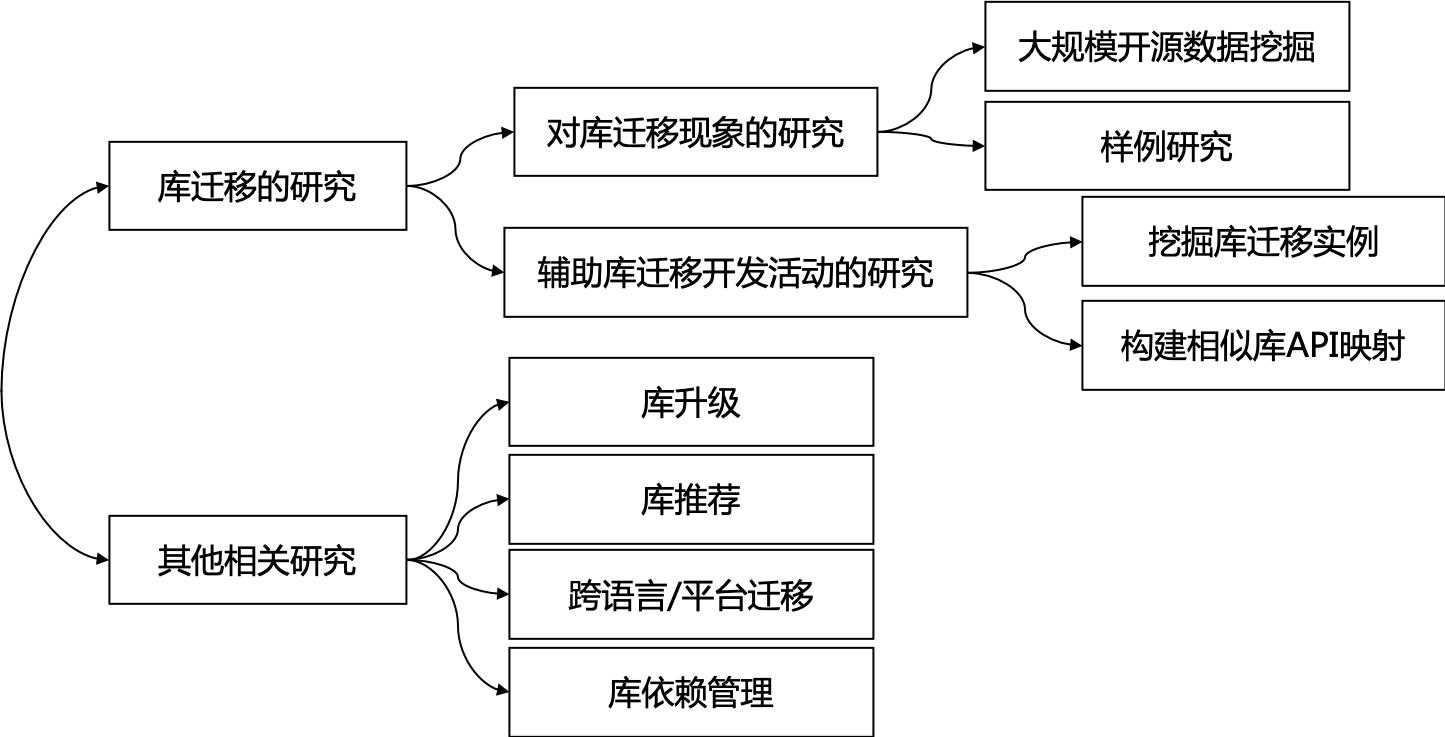
\includegraphics[width=\textwidth]{fig/paper_summary.png}
\caption{相关研究分类}
\label{fig:paper-summary} 
\end{figure}

软件工程学术界中已经存在一些与库迁移有关联的研究。对这些研究的详细分类参见图\ref{fig:paper-summary}。第一类是直接对库迁移进行的研究,包括对库迁移现象本身的研究,和辅助库迁移开发活动的研究。前者主要是利用大规模开源数据或者样例研究等方法,研究开源世界发生过哪些库迁移,库迁移发生的原因,迁移的过程,以及迁移的收益与后果等等。后者则主要是设计一些技术性的方法,来辅助与库迁移有关的开发活动。除了直接对库迁移进行的研究之外,还有不少其他相关研究,这些研究虽然本身研究的对象不是库迁移,但是我们认为他们所研究的问题与库迁移相关,并且使用的方法有可能被应用到库迁移上,因此我们也将其包含在了本综述内。我们会介绍四类其他相关研究:库升级、库推荐、跨语言/平台迁移和库依赖管理。

本文余下部分是这样组织的。首先,第二节介绍了文献收集方法;紧接着,第三节分别从研究的问题、使用的方法技术、提供的数据集和开源工具的角度介绍已有的相关工作;然后,第四节探讨我们对已有工作的看法以及对未来研究的展望;第五节探讨我们对未来可以落地的实际应用的展望;最后第六节总结全文,得出结论。

\section{文献收集和调研方法}
\label{section:survey-method}

% 这一块全部写完之后可能还要再修改
本文对文献的收集和选择,遵循软件工程领域通行的系统性文献综述(Systematic Literature Review)方法\cite{2006ICSE-Budgen-Performing, 2007JournalSysAndSoft-Brereton-Lessons, 2014EASE-Wohlin-Guidelines, 2018EMSE-Ribeiro-Challenges}。
首先,我们将本综述需要覆盖的范围定义为:与库迁移有直接关联,或者潜在可以辅助到库迁移过程的学术研究。
然后,我们在Google Scholar\footnote{\url{https://scholar.google.com/}}和DBLP\footnote{\url{https://dblp.org/}}上检索“Library Migration”关键词,通过阅读论文标题和摘要确定相关性,筛选得到初始论文集合。
随后,我们采用滚雪球(Snowballing)的方法来扩展初始论文集合\cite{2014EASE-Wohlin-Guidelines},对于每篇论文,通过查看全部引用和被引的论文,使用标题和摘要筛选,得到更多的相关论文。
对于可以潜在辅助到库迁移过程的研究,我们仅对每个主题,选择具有代表性的研究进行介绍。
我们选择的论文基本都是在经过同行评审的正规会议或期刊上发表的论文,不过为了保证综述的前沿性,也包括了少量近两年在Arxiv\footnote{\url{https://arxiv.org/}}上发表的预印本论文。

% TODO: 整理一份全部文献的CSV,然后画一些图表
% 简单图表展示,有年份、会议、问题概要即可
通过上述过程,我们一共得到了约40篇论文。表\ref{table:related-work}总结了我们本次综述涉及的所有论文,并按照研究的目的进行了分类。
图\ref{fig:paper-year}和图\ref{fig:paper-conf}分别显示了相关文献在发表年份和会议/期刊上的分布。

\begin{table}[]
    \begin{center}
    \caption{相关文献列表}
    \label{table:related-work} 
	\begin{tabular}{|l|l|l|}
	\hline
	\multicolumn{2}{|l|}{\textbf{研究分类}}                    & \textbf{相关研究} \\ \hline
	\multirow{2}{*}{对库迁移的研究}     & 对迁移现象本身的研究         & \cite{2009SLE-Bartolomei-Study, 2010ICSM-Bartolomei-Swing, 2012WCRE-Teyton-Mining, 2014JournalOfSysAndSoft-Teyton-Study, 2016MSR-Kabinna-Logging, 2018ICSME-Zapata-Towards, 2018EMSE-Kula-Do, 2019Arxiv-Alrubaye-How}      \\ \cline{2-3} 
   	                             & 辅助库迁移开发活动的研究     & \cite{2012WCRE-Teyton-Mining, 2014JournalOfSysAndSoft-Teyton-Study, 2019ICSME-Alrubaye-MigrationMiner, 2011FSE-Zheng-Cross, 2013WCRE-Teyton-Automatic, 2013ICSE-Gokhale-Inferring, 2019ICPC-Alrubaye-On, 2018CASCON-Alrubaye-Automating, 2019Arxiv-Alrubaye-Learning}     \\ \hline
	\multirow{4}{*}{其他相关研究}   & 库升级      & \cite{2005ICSE-Henkel-CatchUp, 2008ICSE-Dagenais-Recommending, 2012FSE-Cossette-Seeking, 2014WCRE-Hora-APIEvolutionMiner, 2018MSR-Lamothe-Exploring, 2018ICSME-Zapata-Towards, 2018EMSE-Kula-Do}      \\ \cline{2-3} 
                                 & 库推荐      &  \cite{2013WCRE-Thung-Automated, 2016ASE-SimilarTech, 2017InfoSciAndTech-Ouni-Search, 2018ICSE-Mora-Which, 2018PROMISE-Mora-An, 2019MSR-Theeten-Import2Vec, 2020TSE-He-Diversified, 2020FSE-Larios-Selecting}    \\ \cline{2-3} 
                                 & 跨语言/平台迁移 &  \cite{2013FSE-Nguyen-Lexical, 2014ASE-Nguyen-Statistical, 2015ASE-Nguyen-DivideAndConquer,2016ICSE-Nguyen-Mapping,2016ICSM-Nguyen-Context,2017ICJAI-Gu-DeepAM,2017ICSE-Phan-Statistical}   \\ \cline{2-3}
                                 & 依赖管理 &  \cite{2017MSR-Kikas-Structure, 2019TSE-Decan-Semantic, 2019MSR-Valero-DiversityMaven, 2019MSR-Dietrich-DependencyVersioning, 2018ICSME-Zapata-Towards, 2018EMSE-Kula-Do}   \\ \hline
	\end{tabular}
	\end{center}
\end{table}


\begin{figure*}[t!]
\centering
	\begin{subfigure}[t]{0.55\textwidth}
        \centering
        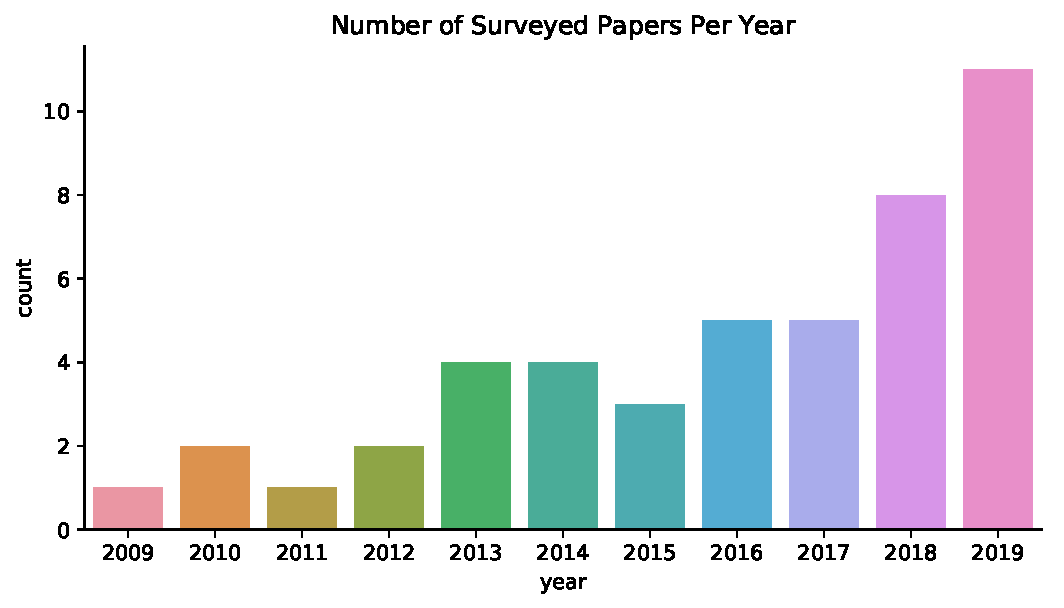
\includegraphics[height=1.4in]{fig/paper_year.pdf}
        \caption{相关论文发表的年份}
        \label{fig:paper-year} 
    \end{subfigure}
    ~
    \begin{subfigure}[t]{0.4\textwidth}
        \centering
        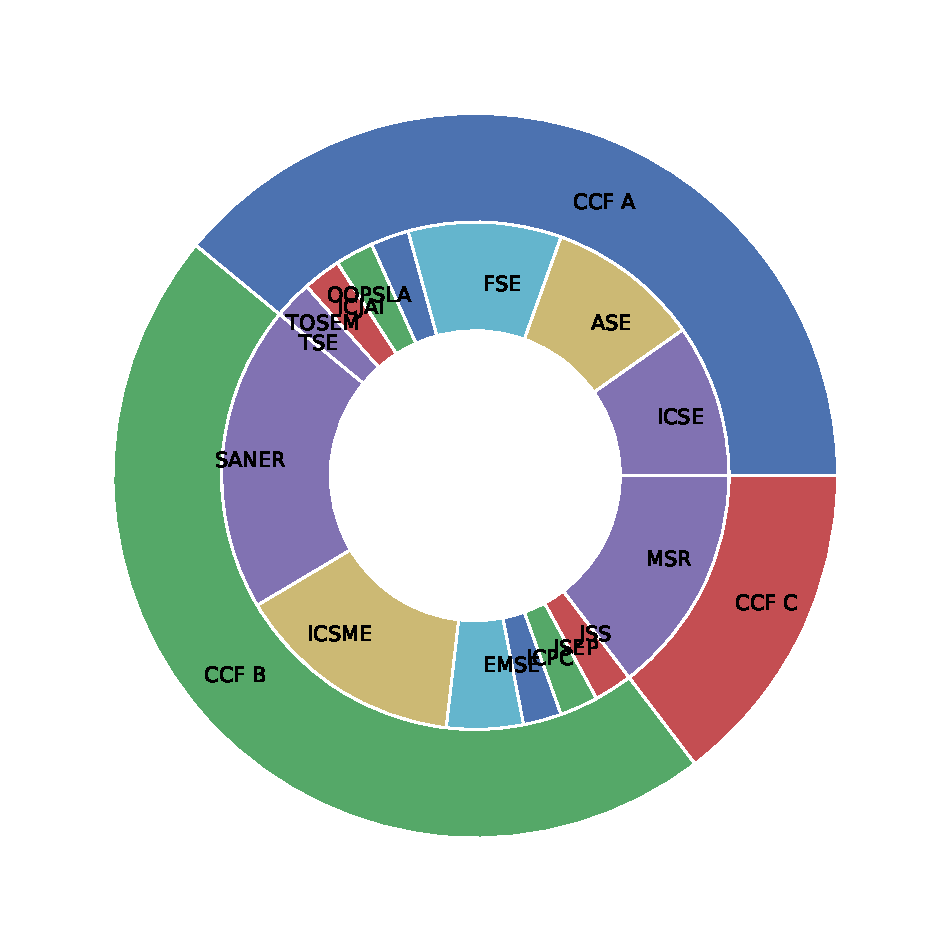
\includegraphics[height=1.4in]{fig/paper_conf_rank.pdf}
        \caption{相关论文发表的会议/期刊}
        \label{fig:paper-conf} 
    \end{subfigure}
\end{figure*}

\section{相关研究介绍}
\label{section:related-work}

\subsection{按研究目的分类}

\subsubsection{对迁移现象本身的研究}

% 每段介绍一篇文章,需要包含该文章的研究问题、研究的意义、研究方法、结果
% case study也放在这

对迁移现象本身的研究主要采用实证研究的方式。\textbf{实证研究}(Empirical Study)是指研究者通过收集和分析实际观察资料来获得结果的研究。在软件工程领域中,实证研究通常会通过收集实际的软件活动数据并对数据进行分析,以及对实际开发者的访谈等形式,得到能够指导软件工程实践的结论。实证研究已经构成了软件工程领域的一个重要组成部分\cite{2002TSE-Kitchenham-Preliminary, 2007ICSE-Sjoberg-Future}。对库迁移现象进行实证研究,不仅可以获得对这一现象的认识,提供对开发者和开发实践的指导,也可以为自动化工具的研发提供思路。

库迁移的实证研究主要包括迁移现状的研究,迁移原因的研究,迁移方法的研究,迁移面临的困难的研究,迁移所需的代价的研究以及迁移造成的影响的研究。

迁移现状方面,Teyton等人\cite{2014JournalOfSysAndSoft-Teyton-Study}在15168个JAVA项目上挖掘迁移规则,发现其中866个项目	($5.57\%$) 曾经发生迁移。
他们进一步将这些项目按照版本数量,代码行数以及开发者数量划分为5959个大型项目($39.3\%$)和9209个小型项目($60.7\%$),发现发生迁移的项目中有593个项目($68.5\%$)属于大型项目,即$9.95\%$的大型项目曾经发生迁移。
说明代码迁移是普遍存在的现象,且大型项目更加可能进行代码迁移。

为了将项目间的迁移可视化,Teyton等人\cite{2012WCRE-Teyton-Mining, 2014JournalOfSysAndSoft-Teyton-Study}利用在海量Java项目上挖掘的迁移规则,构建了迁移关系图。
迁移关系图是一种带权有向图,其中节点是库,从库A到库B的边代表从库A到库B的迁移关系,边的权重表示从库A到库B的迁移发生的次数。
他们针对日志类的库,JSON解析类的库,数据库类的库以及测试类的库构建迁移关系图,将库分为四种类型: 1)迁入远大于迁出的库,2)迁出远大于迁入的库,3)被重要的项目频繁迁入的库,4)迁入和迁出差距不大的库,他们认为第1类库和第3类库是值得推荐的库,第2类库是不值得推荐的库。

%Teyton等人在两项研究中\cite{2012WCRE-Teyton-Mining, 2014JournalOfSysAndSoft-Teyton-Study},利用在海量Java项目上自动化挖掘得到的库迁移实例数据,对日志库、JSON库、数据库等同类相似库比较多的库,构建得到了\textbf{迁移关系图}(Migration Graph)。迁移关系图是一种带权有向图,其中节点是库,从库A到库B的边代表从库A迁移到库B的迁移关系,边的权重表示从库A到库B的迁移实际发生了多少次。Teyton等人还基于这样的迁移关系图,将库分为Gold Rush、Exodus、Challenger和Pong四种类型,用来刻画这个库的特征。比如,这个库是正在有很多项目迁移进去使用它(Gold Rush);还是有很多人正在迁移出去不用它(Challenger);抑或是一个新兴的,大量使用者涌入的库(Challenger);又或是既有迁入,又有迁出(Pong)。研究认为,通过挖掘和分析迁移关系图,可以辅助开发人员做出库迁移决策。


迁移方法方面,Bartolomei等人\cite{2009SLE-Bartolomei-Study, 2010ICSM-Bartolomei-Swing}分别针对Java语言中两种相似的XML库和两种相似的GUI库,探讨了通过设计API封装库,进行自动化迁移的可能性。他们通过研究了已有的API封装库,总结了多种用于迁移的设计模式。一个重要的发现是,即使两个库表面上看上去功能非常相似,但是由于功能和实现细节上的种种微妙差别,使得设计和实现这样的API封装库并不容易。

迁移面临的困难方面,Kabinna等人\cite{2016MSR-Kabinna-Logging}通过挖掘14个没有成功进行迁移的问题报告,将迁移失败的原因总结为4个方面: 1)开发者没有达成共识,2)没有人进行代码提交,3)开发者希望等待更好的替代库,4)项目的依赖关系导致迁移无法进行。
这说明迁移并不是能够轻易决定的事情。

迁移所需的代价方面,Alrubaye等人\cite{2019ICPC-Alrubaye-On}通过计算迁移开始的代码提交与迁移结束的代码提交,发现迁移平均需要2-42天的时间,且不同类型的迁移耗时不同。
这说明迁移是耗时的过程。

迁移造成的影响方面,Kabinna等人\cite{2016MSR-Kabinna-Logging}通过挖掘33个发生日志类库迁移的代码项目,发现其中24个项目在迁移后半年内平均遇到了2个与迁移相关的缺陷。
他们同时选择了3个由于性能方面原因进行库迁移的项目,运行迁移前后的代码,发现其中的2个项目在迁移后性能得到了显著提升。
Alrubaye等人\cite{2019Arxiv-Alrubaye-How}通过在迁移前后的代码文件上计算相应的量度,发现代码迁移能够提升提升软件的质量与可读性。
总的来说,代码迁移能够提升项目的运行效率与代码质量,但是迁移的过程也可能会引入部分缺陷。

% 详细部分我准备读完这篇论文再写
%Cossette等人在一项研究中\cite{2012FSE-Cossette-Seeking},深入研究了不同版本的Java库之间的API的不同,以及当时的自动化方法在实际Java库升级上的表现。

%\cite{2016MSR-Kabinna-Logging}
%Kabinna等人在一项研究中,出于更好地研究日志库的动机

% \textbf{迁移的原因}。

% \textbf{迁移中会遇到的困难}

% \textbf{开发者如何做迁移}

% \textbf{迁移的副作用}

\subsubsection{辅助迁移实践的研究}

辅助库迁移实践的研究有以下几类:库迁移实例挖掘、推荐迁移替代库、以及辅助代码迁移活动。

%1)先说明库依赖挖掘方法是什么,为什么基础。

%2)库依赖挖掘目前主流的两种方法:包管理器文件分析、静态代码分析。分两段介绍。再起一段说明两者结合的文章的方法。

\paragraph{库迁移实例挖掘}
目前辅助迁移实践的研究主要采用数据驱动(data-driven)的思路,也就是利用开源社区中已经存在的迁移及其相关数据来解决各种问题。
因此,本文首先介绍如何从开源社区中获取库迁移有关的数据。

Teyton等人\cite{2012WCRE-Teyton-Mining}提出了一种基于版本间依赖库变化,构建库迁移关系图的方法。
在他们对提出的方法进行实证研究的时候,他们采用了分析Java语言下的Maven包管理器的POM文件的方法,进行每个版本的库依赖信息的提取。
在POM文件中,一个依赖库包含三个信息,分别是:依赖库所属的组织名称、依赖库名称、依赖库版本号。
该文章使用依赖库组织名称与依赖库名称进行同一个依赖库的唯一标识,而同一依赖库的不同版本被认为是相同的依赖库,这在研究库迁移的环境下是可取的。

%\marginpar{依赖库的信息好像是4个,还有scope? -Hanmin Qin}
%scope那个在库迁移问题中应该不是很关键,它只是定义了使用这个库的方式,比如是仅编译时使用,还是一起打包,还是仅测试时使用等等。- Yulin

Teyton等人在后面的研究中\cite{2014JournalOfSysAndSoft-Teyton-Study},提出了另一种识别软件项目内使用的依赖库的方法,这种方法基于静态代码分析,识别软件代码中使用的标识符,通过确认标识符所属的依赖库,来确定该软件项目使用了哪些依赖库。
这种方法可以与包管理器无关,无论使用了哪种包管理器,或是没有使用包管理器,都可以用同样的代码分析方法进行依赖库的挖掘。
但是这种方法也会遇到其他的问题,首先在使用这种方法之前,需要构建一个标识符到依赖库的映射关系,该文章是通过分析一个库的所有版本的发布包,来获取一个依赖库内可能包含的所有标识符集合。
在获取了所有依赖库的标识符集合后,可能会遇到不同依赖库之间标识符冲突的问题,导致这种问题的可能原因之一是某个完整的依赖库引用了一个单独的组件,此时该组件的所有标识符都存在于完整依赖库的标识符集合中,这种情况下该文章采取的方法是,将该单独组件移出依赖库列表,只记录完整依赖库的信息。
另一种可能的原因是,依赖库A在使用其他依赖库B的时候,自主重新定义了B中的部分标识符,这种情况下该文章采取的方法是删除这部分互相冲突的标识符。

%\marginpar{似乎应该提及跨版本的项目迁移,就是A版本首先引入新的库,然后B版本移除旧的库? -Hanmin Qin}
%这个小节还只是在说如何分析软件依赖了什么库,还没涉及迁移 -Yulin

Alrubaye等人在近期的三篇研究当中\cite{2019ICSME-Alrubaye-MigrationMiner,2019ICPC-Alrubaye-On,2018CASCON-Alrubaye-Automating},提出了基于包管理器与静态代码分析结合的方法。
他们的工作中存在一个步骤,希望寻找出软件项目发生库迁移的具体时间段,而如果仅依靠包管理进行依赖库的分析,会无法正确识别出迁移完成后未删除旧的依赖库的情况。
因此,他们在分析出包管理器内加入了新的库后,逐个扫描每个版本的代码,确认旧的依赖库完全不被使用的时间,由此确认软件项目进行库迁移的时间段。

% 加一段总结

\paragraph{推荐迁移替代库}
在拥有了相关的数据之后,比较容易想到的思路是利用已有数据,对新项目的迁移决策进行推荐。

%1)先说明主要的推荐方法就是库迁移规则挖掘方法,库迁移规则挖掘方法是什么、有什么用。

目前,在以库迁移为目标的替代库推荐研究中,使用得最多的方法是通过挖掘已有软件项目的开发历史,获取库迁移规则,并基于这些已有规则进行推荐的方法,以下我们称这种方法为库迁移规则挖掘方法。
库迁移规则挖掘方法不仅是推荐迁移替代库的一个重要核心方法,更是许多库迁移研究中的基础问题。
要对库迁移现象开展任何方面的研究,都必须要得到一定数量的在真实软件开发中进行的库迁移实例,作为开展更深入研究的基础。
幸运的是,任何一个使用Git作为版本控制系统的项目都会包含完整的项目开发历史信息,并且开源软件的蓬勃发展使得研究者可以从互联网上获得大量开源的项目开发数据。
不幸的是,从这些开发历史数据中挖掘得到真实的库迁移实例不是一个简单的问题。
首先,已有研究的证据显示库迁移并不经常发生\cite{2012WCRE-Teyton-Mining, 2014JournalOfSysAndSoft-Teyton-Study},从而要获得具有较大数量的迁移实例,必须从海量开源项目和开源库中进行自动化挖掘,这个过程通常会涉及到数万个项目和数万个库。
此外,由于不同项目进行库迁移所涉及的开发活动都会有所不同,从而很难对库迁移行为给予一个严格的形式化定义,使得目前的自动化挖掘方法都是启发式的推断方法。
通常,一个自动化的挖掘方法,会通过分析项目使用的第三方库信息随时间的变化,并结合静态代码分析来推测项目中是否存在库迁移。
我们可以从两个角度来评判库迁移规则挖掘方法,一是库迁移规则挖掘的准确率(Precision),亦即发现的库迁移实例有多少是真实的库迁移实例;二是库迁移规则挖掘的召回率(Recall),亦即是否能够尽可能多地不要遗漏真实的库迁移实例。
然而,由于我们难以在超大规模数据上获得库迁移的完整真实情况(Ground Truth),从而对召回率的评测相当困难,已有研究一般只能采用某种方法来估计召回率。

%2)库迁移规则挖掘分为两个步骤:迁移规则发现、过滤无效规则。分两段说明各文章在这两个步骤上的做法、有何改进、有何不足。

库迁移规则挖掘方法在已有研究中,主要分为两个步骤进行:迁移规则发现、过滤无效规则。
迁移规则发现是指,从软件项目的开发历史数据中,推断出可能发生过的库迁移,从而将其作为候选的库迁移规则,这一步骤的主要目标是尽可能地提高迁移规则挖掘的召回率。
过滤无效规则是指,在前一个步骤中发现的迁移规则,可能存在被误判为库迁移的规则,需要一系列手段进行过滤,提升迁移规则挖掘的准确率。下面本文就这两个步骤,分别总结已有研究所使用的方法。

Teyton\cite{2012WCRE-Teyton-Mining}等人,最先提出了一种构建迁移关系图的方法,来挖掘已有项目中可能发生过的迁移。
他们先假设能找到一个项目的每个版本依赖的库,由此能分析出每个版本之间新增和删除的库,最终在每个版本删除的库到新增的库之间就能建立一个迁移关系。
Teyton等人提出的方法,提供了最基本的从已有项目历史中挖掘迁移规则的思路,即根据版本间依赖库的变化,推断可能发生的迁移。
但这种方法存在一些问题会影响挖掘的召回率和准确率。
如果项目引入新依赖库的版本和移除旧依赖库的版本不是同一个版本,这种简单方法会无法挖掘出这种迁移规则,导致召回率下降。
另外,如果在删除旧依赖的同时引入了替代库以外的其他依赖库,会导致错误挖掘出旧依赖库到某些无关的依赖库的迁移规则,导致准确率下降。
后来的研究对这些问题分别提出了一些改进算法。

Teyton\cite{2013WCRE-Teyton-Automatic}等人在后来的工作中,研究如何为可相互替代的库之间构建API的映射,这篇工作同时还对之前的迁移规则挖掘方法进行了改进,提升了方法的召回率。
这篇工作假设,库迁移不是发生在一个版本之内,而是在几个版本构成的一个时间区间内完成的。
因此,如果要认为库A可能迁移到了库B,需要满足以下条件:在版本i,j($i \textless j$)之间,库A存在于版本i的依赖库集合中但不存在于版本j的依赖库集合中,且库B存在于版本j的依赖库集合中但不存在于版本i的依赖库集合中。
这种方法解决了引入新库后若干个版本才移除旧库的情况下,召回率下降的问题。
在Teyton\cite{2014JournalOfSysAndSoft-Teyton-Study}等人后续的工作中,依然是使用了这种算法进行初步的迁移规则挖掘。

然而上述方法在提高召回率的同时,可能挖掘出了大量的无关规则,降低了准确率,因此部分研究在大量发现迁移规则后,会进行过滤无效规则的处理以提升准确率。
部分研究在数据量不大的情况下,为了更好地开展后续的实证研究,对迁移规则进行了人工的筛选,去除了大量false positive的迁移规则。
Teyton等人在\cite{2012WCRE-Teyton-Mining}中参考了commit log来进行人工筛选,他们发现项目发生迁移时,会在commit message中提到相关库的信息。
Teyton等人在另一篇工作中\cite{2014JournalOfSysAndSoft-Teyton-Study}采用的是通过咨询软件专家来进行人工筛选。
还有部分研究采用了设置支持度阈值进行过滤的方法,这类方法的核心思想是,记录每条迁移规则出现的总次数,并计算每条迁移规则的支持度,最后仅保留支持度大于指定的阈值的规则。
Teyton等人在\cite{2012WCRE-Teyton-Mining}中除了采用人工筛选方法外,也使用了支持度的方法,他们为一条库A迁移到库B的迁移规则m计算了两种支持度,最终m的支持度以两种中较小的计算。
两种支持度的计算都以规则m出现在的项目版本的数量为分子,第一种支持度的分母是出现了从库A迁出到其他库的项目版本数量,第二种支持度的分母是出现了从其他库迁入到库B的项目版本数量。
Alrubaye等人\cite{2019ICSME-Alrubaye-MigrationMiner}也使用了类似的支持度算法,但是他们采用的支持度的分母是,以库A为源的所有迁移规则中出现次数最多的规则的次数。
同时,他们还采用了结合代码分析的方法,他们分析了每个commit涉及的API修改,如果不存在库A到库B的API修改,则说明该规则是一条无效的规则,因此可以过滤掉该规则提高准确率。

% 3)补充其他推荐迁移替代库的方法

其他获取库迁移规则的方法中值得一提的是,实证研究\cite{2016MSR-Kabinna-Logging}采用了在开发管理和问题追踪软件JIRA\footnote{\url{https://www.atlassian.com/software/jira}}上进行关键词检索的方法来获得库迁移实例。
它能这么做的原因是作为它的研究对象的Apache基金会项目都使用此软件来管理开发日志,但这不是一个通用的方法。

% 补充一段总结

\paragraph{辅助代码迁移活动}
在通过库迁移规则挖掘方法得到实际项目的库迁移实例数据后,一个很自然的想法就是探索如何能够使用已有项目的历史数据,来辅助当前正在进行的库迁移。
例如,在实际将对一个库的调用代码修改成对另一个库的调用代码的过程中,如果能够告诉开发人员另一个库的哪些API功能与这个库的某个API类似,那么就能提升开发人员进行代码修改的效率。

%1)说明API映射方法的研究的用途

出于此动机,有研究人员先后试图探索了如何自动化地在相似的库之间建立API的映射关系的问题\cite{2011FSE-Zheng-Cross, 2013WCRE-Teyton-Automatic, 2013ICSE-Gokhale-Inferring, 2019ICPC-Alrubaye-On, 2018CASCON-Alrubaye-Automating, 2019Arxiv-Alrubaye-Learning}。在一项早期研究中,Zheng等人\cite{2011FSE-Zheng-Cross}提出了基于搜索引擎获取信息的API映射方法,并使用了一些信息检索相关的技术。
之后的研究渐渐转移到使用库迁移历史信息来建立API映射。
这么做的原因在于,在库迁移的过程中,开发人员必然会留下把一个库的API替换成另一个库的API的历史数据,那么就自然可以利用这些历史数据。
Teyton等人在\cite{2013WCRE-Teyton-Automatic}中首先基于库迁移历史数据,利用笛卡尔积建立二部图并在图上使用某种图匹配算法\cite{2002ICDE-Melnik-Similarity},用于得到相似库之间的映射关系。
之后,Alrubaya等人在一系列工作中\cite{2019ICPC-Alrubaye-On, 2018CASCON-Alrubaye-Automating, 2019Arxiv-Alrubaye-Learning},综合使用了文档挖掘、信息检索、片段排序和机器学习等方法,大幅提升了匹配的准确率。
然而,根据我们所调研的结果,目前似乎并没有研究报告了这一API映射算法在实践中,究竟能对开发人员起到何种程度的帮助。

%2)每段介绍一篇涉及API映射的文章,说明所使用的方法,如有针对某种问题的改进也要特别说明

Zheng等人\cite{2011FSE-Zheng-Cross}提出了一种基于搜索引擎的API映射方法,他们的方法可以在搜索引擎中查找出指定API在指定的库中最可能的替代API。
首先,他们构造若干个搜索请求,请求中包含需要被替换的API名称和替代库的名称,以此请求搜索引擎的结果。
在搜索结果中,他们需要过滤出与被替代库相关的结果,他们的方法是,构造一个包含替代库全部API名称的字典,如果搜索结果的标题或摘要中包含被替代库的API名称,则被保留。
在所有的相关请求结果中,他们需要挖掘出最相关的候选API,他们的方法是,将每个请求的所有相关结果中出现的替代库的API名称构造成一个文档,多次搜索请求则可以获得多个这样的文档,再对这组文档中的每个替代库API计算TF-IDF值,得分最高的即是最相关的替代API。
这种方法是早期的研究中对API映射问题的一个简单尝试。

Teyton等人\cite{2013WCRE-Teyton-Automatic}提出了一种基于挖掘开发历史数据的API映射方法。
在推荐迁移替代库小节中,我们描述了该工作如何基于开发历史数据挖掘库迁移规则,以及确定库迁移发生的时间段。
在此基础上,该研究还提出了如何基于开发历史数据,在特定的库迁移规则和时间区间内,挖掘API映射规则的方法。
他们首先针对每个commit使用diff工具分析变更的文件,记录下每个文件的diff中被删除的行号以及新增的行号。
然后他们对该文件的上一个版本进行静态代码分析,提取出被删除行号中相关的API标识符,同时在该文件的当前版本的静态代码分析中,提取出新增行号的相关API标识符,由此得到了该commit删除的API集合和新增的API集合。
他们对上述两个集合的API做了笛卡尔积,得到候选的API映射关系,再将对指定时间段中全部commit分析得到的候选API映射关系合并成一个带有边权重的二部图,边权即为该API映射关系出现的次数。
最后,他们使用relative similarity\cite{2002ICDE-Melnik-Similarity}方法,对二部图上的边进行过滤,去除了部分false positive,提高准确率。

Gokhale等人\cite{2013ICSE-Gokhale-Inferring}提出了一种基于比较相似功能的函数的执行流中调用的API来挖掘API映射关系的方法。
该方法主要参考了四种因子来推断不同执行流中多个API之间的映射关系。
第一种因子是API在该执行流中被调用的频率,相似功能的不同执行流中,API被调用的频率应该接近。
第二种因子是API在执行流中被调用的位置,相似功能的不同执行流中,API被调用的位置应该接近。
第三种因子是API附近的其他API,如果我们已经能确认一组API映射关系,而且在这些API附近经常能发现其他API,则其他的API之间也可能有映射关系。
第四种因子是API的名称,API名称中通常包含一些关键信息,如果名称相似,则很有可能功能相似。

Alrubaye等人在两篇工作中\cite{2018CASCON-Alrubaye-Automating}\cite{2019ICPC-Alrubaye-On}一共对4种挖掘API映射的方法进行了比较。
其中一种方法,在文中被简称为FC,即为上文描述的Teyton等人\cite{2013WCRE-Teyton-Automatic}提出的方法。
第二种方法被简称为FS,是基于API相似度进行的度量,最终保留相似度最高的API映射关系,其中API相似度的算法引用的是Nguyen等人在\cite{2010OOPSLA-Nguyen-Graph}中使用过的算法,主要参考因子有方法名相似度、返回类型相似度、参数列表相似度。
第三种方法被简称为MC,是FC的简化版,为每个API仅保留边权最高的一组API映射关系。
第四种方法被简称为SA,是Alrubaye等人在\cite{2019ICPC-Alrubaye-On}中提出的新方法。
SA是基于挖掘不同的多对多映射关系中的共同一对一映射或是一对多映射,来达到挖掘API映射的目的。
SA算法是一个迭代的过程,每轮迭代中,先把一组片段进行排序,其中一个片段包含被删除的API集合与被添加的API集合以及这种删除与添加API的模式在不同代码变更位置中出现的次数。
片段排序优先考虑被删除的API集合与被添加的API集合中API的数量,API数量少的片段排在前面,其次考虑该片段出现的次数,次数多的排在前面。
接下来按顺序两两比较片段,如果两个片段的被删除API集合与被添加API集合中都存在共同的API,则将原来的两个片段移出列表,并加入新的三个片段,其中一个是由共同的API组成的片段,其余两个是由原来的两个片段移除了共同的API后形成的片段。
加入新片段后,重新排序开始新一轮迭代。
如果在某轮迭代中无法加入新的片段,但是仍然存在多对多的映射关系片段的话,则将排序靠前的多对多映射关系片段中的被删除API与被添加API两两计算相似度,取相似度最高的一对API作为新的片段加入列表,重新排序开始新一轮迭代。
其中相似度的计算方法是使用API的文档的文本相似度。
最后在\cite{2019ICPC-Alrubaye-On}中,对这四种方法进行了比较,他们的F-Measure分别是FC:53.8\%,MC:46.5\%,FS:63.3\%,SA:75.2\%。

% 补充一段总结

\subsubsection{其他研究}

\paragraph{库升级}

%库升级的英文名再斟酌一下

一种与库迁移非常相关的研究主题是库升级(Library Upgrade)。
在已有文献中,部分英文文献也将库升级称为“Library Migration”,但是他们研究的主题是,同一个库的不同版本之间进行变更。
在对原因、难点等现象本身的研究方面,库迁移与库升级存在较大差别,但是在一些自动化辅助工具的研究方面,库升级可以看做是库迁移的一种特例,所使用的技术也存在相通性。
因此,本小节将对库升级的自动化辅助技术相关的工作进行总结。

在早期的工作中,Henkel等人\cite{2005ICSE-Henkel-CatchUp}提出了一种基于录制重构代码的操作,并将录制下来的操作重新应用于其他待重构代码上的辅助库升级的技术。
他们设计了一种集成开发环境(IDE)的插件,库的开发者可以在安装了这种插件的IDE内,进行库升级的重构工作,插件会记录他们执行的重构操作到文件中。
当把这些记录了重构操作的文件连同升级的库一起分发给库的使用者时,库使用者可以在他们的代码中需要重构的位置,重新执行录制好的操作来实现自动化库升级。

在Dagenais等人\cite{2008ICSE-Dagenais-Recommending}的工作中,他们发现在库本身的代码中,包含许多对库自己提供的API的使用,而在不同的库版本之间,如果某个API发生了变化,那么这些使用了库自身API的代码也会发生相应的变化。
因此他们提出了一种基于挖掘库本身的版本控制系统的历史,获取每一次提交中发生变化的调用库本身API的代码,来挖掘库升级时的API变化规则。
同时,他们还定义了一些此种挖掘方法会遇到的问题并加以解决,比如挖掘到多个不同的变化规则时,他们会计算不同规则的支持度并将其展示给用户来辅助用户判断;当某个API发生了多次变化时,他们会构建出变化链,从而忽略中间的变化,直接给用户推荐最终的变化方式。
他们还说明了这种方法也存在缺陷,某些根层次的API可能只会被库使用者调用,不会被库本身调用,那么这些API的变化就无法被挖掘出来。

在Hora等人\cite{2014WCRE-Hora-APIEvolutionMiner}的工作中,他们通过挖掘库使用者的版本控制系统的历史,来获取API变化后的重构方法。
他们对挖掘得到的API调用方法进行了一定的归一化处理,将一些参数、变量等用通配符代替,使得类似的调用方法被归约为一种调用方法。
在一处代码变化中,可能包含多个API调用方法的变化,比如删除了某API和添加了另一API。
他们将一处代码变化视为频繁模式挖掘中的事务(transaction),而每一项API调用方法变化视为项目(item)。
频繁模式挖掘算法可以在一组事务中,挖掘出频繁出现的项目子集,这样一组项目子集,就可以认为是有效的API重构方法集合。

最后,在Lamothe等人\cite{2018MSR-Lamothe-Exploring}的工作中,他们探究了上述工作在Android的API变化中是否具有实际价值。
他们在研究中总结到,自动化的辅助库升级技术,主要有基于文档挖掘的、基于提交信息挖掘的和基于代码变更挖掘的的技术。
他们通过对6个Android版本的文档的分析发现,大部分API的变更(包含删除和弃用)都可以在文档中找到对应的替代API信息,能找到替代API的比例从51\%到98.4\%不等,其中仅有一个版本是51\%,其他五个版本均在80\%以上。
同时他们还发现,有26\%的API变更无法找到任何替代API,可能是这项功能被根本性地移除了。
他们还验证了基于代码变化挖掘API变更方法的有效性,他们发现基于文档的信息可以挖掘出119个API变更方法,而基于代码变化信息仅能挖掘出53个,其中仅有5个是只在代码变化中能挖掘出来的,其余均与文档中挖掘出来的一致。
他们还验证了基于代码变化挖掘的方法的基础假设是否有效,即API的删除与添加是否会存在于同一个提交中。
他们发现,有57.3\%的提交无法确认被删除的API被替代成了其他的API。
他们还发现,替代API被引入Android的版本往往早于原API被弃用或删除的版本,但有三个API的替代API是在后续版本才本引入Android,同时Android中存在大量被弃用的API没有被删除。
这些复杂的现实情况表明,无论是基于挖掘库本身的版本控制历史,还是挖掘库使用者的版本控制历史,都会存在大量的复杂情况导致挖掘效果下降。
但是这种效果下降,仅是在Android上的发现,在其他大范围的项目内表现如何还需要进一步研究。
同时这些研究也是针对库升级的场景来进行的,如果在库迁移的场景下,这些复杂的情形是否会大量存在,也需要重新在库迁移的场景下进行验证和研究。

\paragraph{库推荐}
除了以上所说的推荐库迁移替代库有关的研究之外,也存在直接根据一个项目正在使用的库来推荐相关库的研究\cite{2013WCRE-Thung-Automated, 2017InfoSciAndTech-Ouni-Search,2019MSR-Theeten-Import2Vec}。这一类研究的假设在于,如果一个项目使用的依赖库与其他项目类似,那么这个项目也很可能会用到其他项目也用到的库。为了达成精准的推荐,这类研究使用了多种思路,包括应用推荐系统中著名的关联规则挖掘和协同过滤算法\cite{2013WCRE-Thung-Automated}、搜索和优化算法\cite{2017InfoSciAndTech-Ouni-Search}、使用Word2Vec学习特征向量\cite{2019MSR-Theeten-Import2Vec}等。然而,也有研究指出,上述研究不仅存在严重的面向“热门库”的偏好,且对开发者的实用性存疑\cite{2020TSE-He-Diversified}。然而,相关研究的解决方案思想和评测方法,在库替换推荐的场景下依然有借鉴价值。

此外,值得一提的是,Chen等人探索了如何自动化地在不同语言间寻找相似技术\cite{2016ASE-SimilarTech}。
此文利用Stack Overflow网站上问题标签数据之间的语义关联性,在标签上挖掘相关库的标签,并在整个标签上训练Word2Vec模型,从而自动地学习到了库的标签的语义相似性。
这个方法的优势在于,没有对库的编程语言和运行环境做出任何假设,而是仅仅依赖开发者在问答网站上生成的标签来作答,从而能够有效地推荐到不同语言的相似库,并且能获得较好的效果(81\%准确率)。

最后,也有研究者探索了开发者在选择库时所看重的不同因素\cite{2018ICSE-Mora-Which, 2018PROMISE-Mora-An, 2020FSE-Larios-Selecting}。
Mora等人\cite{2018ICSE-Mora-Which, 2018PROMISE-Mora-An}采用众包网站的形式询问开发者在选择库的时候会在意的因素,以及这些因素与指标的关联性。他们发现,开发者最关心与库的性能、流行度和安全性有关的指标,但是不同领域的开发者对不同指标的看重程度不同。
Larios等人\cite{2020FSE-Larios-Selecting}采用对软件工程师进行访谈的形式总结开发者在选择库的时候会考虑的因素。他们对16个不同领域和不同工作经验的开发者访谈后,总结了26种不同的因素,并归类为技术类、人因(human-factors)类和经济类三大类,并对每一种因素都进行了详细的诠释,深度大大超出了前述工作。
这些研究中所发现的因素,可能也会与库迁移有关,因此可以作为探索库迁移研究的出发点。

\paragraph{跨语言/平台迁移}
还有一类研究致力于解决这样一类问题:将一个编程语言写的项目翻译成另一种编程语言写的项目\cite{2013FSE-Nguyen-Lexical, 2014ASE-Nguyen-Statistical, 2015ASE-Nguyen-DivideAndConquer,2016ICSE-Nguyen-Mapping,2016ICSM-Nguyen-Context,2017ICJAI-Gu-DeepAM,2017ICSE-Phan-Statistical}。在这类问题中,除了语法和语义上的转换外,还需要针对这两类语言中使用的不同标准库,在API之间建立映射和设计自动转换方法。已有研究通常会使用人工智能相关技术,并且借助机器语言翻译领域的最新进展来解决此类问题。这类研究中关于如何在不同语言的库之间建立API的部分,对辅助库迁移的开发活动也有潜在参考价值。

\paragraph{依赖管理}
最后,有相当多的研究还聚焦于进行依赖管理相关的各种其他问题。随着类似NPM这样的包管理器的流行和开源库数量的指数增长,开发者在如何管理项目所使用的库上遇到了不少困难。例如,开发者很可能在不知情的情况下使用了带有安全漏洞的库\cite{2018ICSME-Zapata-Towards};使用的库没有遵循Semantic Versioning使得升级库引入了新的Bug \cite{2019TSE-Decan-Semantic};甚至使用的库可能会被其维护者移除\cite{2017MSR-Kikas-Structure};等等。为了辅助开发者更好地进行软件供应链的管理,近年来出现了大量对于软件依赖管理的研究,例如研究库之间的依赖网络如何演化\cite{2017MSR-Kikas-Structure};开发者对Semantic Versioning的使用情况\cite{2019MSR-Dietrich-DependencyVersioning,2019TSE-Decan-Semantic};开发者如何升级自己的库依赖\cite{2018ICSME-Zapata-Towards,2018EMSE-Kula-Do};等等。

%\subsubsection{其他相关研究}

%(秦汉民)

% 库升级相关研究和其他觉得有关的研究放在此处
% 每段介绍一篇相关研究即可

%\marginpar{你们觉得这个方向靠谱吗?靠谱我继续写}

%库迁移的实质是从某个库迁移到API不完全相同的另一个库,与之紧密相关的是从某个库的特定版本迁移到API不完全相同的另一个版本。Kim等人\cite{DBLP:conf/wcre/KimPW05}定义了8个相似性量度以检测项目不同版本间相同的函数。Wu等人\cite{DBLP:conf/icse/WuGAK10}在相似性量度的基础上考虑了函数之间的调用关系。Xing等人\cite{DBLP:journals/tse/XingS07}则是从代码的修改历史出发挖掘不同版本间相同的函数。此类研究的很多方法都能够作为库迁移研究的参考,例如基于代码修改历史的挖掘方法能够用于库迁移检测,而基于相似性度量的方法能够用于库迁移API映射问题。

\subsection{使用或提供的数据集概述}

%(秦汉民)

% 概述各个论文使用了什么样的数据集,或是提供出了什么样的数据集
% 每段介绍一个数据集,包括如何获取该数据集、该数据集提供的数据内容、被哪些文章如何实际使用过或是介绍可能的使用用途。

库迁移规则的开源数据集主要包括 \cite{library2014} 以及 \cite{library2019}。
数据集\cite{library2014}由Teyton等人\cite{2014JournalOfSysAndSoft-Teyton-Study}通过挖掘GitHub上15168个项目得到,包括329个库迁移规则。
数据集\cite{library2019}由Alrubaye等人\cite{2019ICSME-Alrubaye-MigrationMiner}通过挖掘大约321K开源项目得到,包括3978个库迁移规则。


库迁移API映射的开源数据集主要包括 \cite{API2013} 以及 \cite{API2018}。

Teyton等人\cite{2013WCRE-Teyton-Automatic} \cite{API2013} 通过挖掘11598个来自GitHub, GoogleCode和Sourceforge的JAVA项目得到4种迁移关系下107个函数对应关系。
对于每个对应关系,该数据集提供相应的Javadoc以及迁移实例。
该数据集被Alrubaye等人\cite{2019ICSME-Alrubaye-MigrationMiner}使用。

%\begin{comment}
\begin{table}  
    \begin{center}
    \caption{数据集\cite{API2013}内容举例}
    \label{table_API2013} 
    \begin{tabular}{| c | c | c |}
        \hline 
        迁移前的库 & 迁移后的库 & 迁移出现的次数  \\
        \hline
        commons-io  & guava & 21 \\
        commons-lang  & guava & 40 \\ 
        json & gson & 28 \\
        mockitio  & jmock & 18 \\
        \hline
    \end{tabular}
    \end{center}
\end{table}
%\end{comment}

Alrubaye等人\cite{2018CASCON-Alrubaye-Automating} \cite{API2018}通过挖掘57447个JAVA项目得到14种迁移关系下331个函数对应关系。
(原论文使用的数据集和作者开源的数据集有所不同,只有12种迁移关系下303个函数对应关系)
对于每个代码片段,该数据集提供相应的commit信息。
为了便于复现,该数据集同时提供得到以上对应关系所用的8935个代码片段。
相比\cite{API2013},该数据集考虑了多个函数向多个函数的迁移,但是没有提供相应的Javadoc。
该数据集被Alrubaye等人\cite{2019ICPC-Alrubaye-On} \cite{2019Arxiv-Alrubaye-Learning}使用。

\begin{comment}
\begin{table}  
    \begin{center}
        \caption{数据集\cite{API2018}内容举例}
        \label{table_API2018} 
        \begin{tabular}{| c | c | c | c |}
            \hline 
            迁移前的函数 & 迁移后的函数  & 迁移关系的出现次数  \\
            \hline
            org.testng:testng:xxx & junit:junit:xxx & 71 \\
            commons-logging:commons-logging:xxx & org.slf4j:slf4j:xxx & 54 \\
            org.easymock:easymock:xxx & org.mockito:mockito:xxx & 52 \\
            org.json:json:xxx & com.google.code.gson:gson:xxx & 30 \\
            com.google.code.gson:gson:xxx & com.fasterxml.jackson.core:jackson:xxx & 23 \\
            com.google.collections:google-collect:xxx & com.google.guava:guava:xxx & 19 \\
            commons-httpclient:commons-httpclient:xxx & org.apache.httpcomponents:httpclient:xxx & 18 \\
            org.slf4j:slf4j-api:xxx & log4j:log4j:xxx & 14 \\
            net.java.dev.jets3t:jets3t:xxx & com.amazonaws:aws-java-sdk:xxx & 12 \\
            org.hibernate:hibernate-core:xxx & org.slf4j:slf4j:xxx & 11 \\
            com.googlecode.json-simple:json:xxx & com.google.code.gson:gson:xxx & 10 \\
            commons-lang:commons-lang:xxx & org.slf4j:slf4j-api:xxx & 8 \\
            javax.faces:jsf-api:xxx & org.glassfish:javax.faces:xxx & 5 \\
            org.openrdf.sesame:sesame:xxx & org.eclipse.rdf4j:rdf4j:xxx & 4 \\
            \hline
        \end{tabular}
    \end{center}
\end{table}
\end{comment}

\begin{figure}
\centering
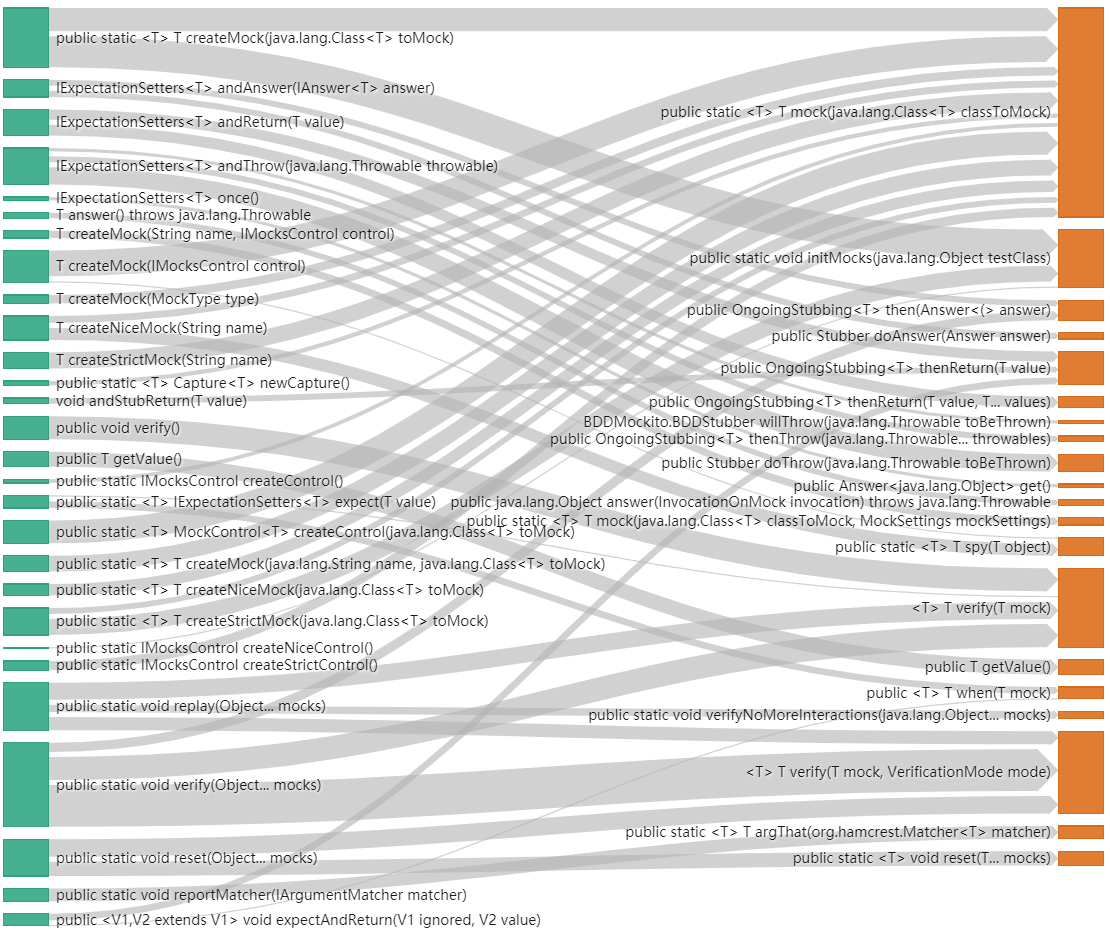
\includegraphics[width=\textwidth]{fig/alrubaye_dataset.png}
\caption{数据集\cite{API2018}内容举例}
\label{fig:api-2018} 
\end{figure}

\subsection{开源工具概述}

%(徐玉麟)

% 概述有提供开源工具的文章提供了什么样的工具,有什么功能,输入输出是什么
% 每段介绍一个工具

Hora\cite{2015ICSME-Hora-Apiwave}等人演示了工具Apiwave,Apiwave可以展示GitHub上前650个流行Java框架、库对API的使用情况,它可以展示这些项目使用的API的流行程度和API的迁移情况。
其中API的流行程度展示了每个API、API所属包、依赖库被使用的次数,还包含该API在时间维度上被新增使用和删除使用的情况。
API迁移情况包含了每种迁移规则发生的次数,以及每种迁移规则对应的迁移实例代码。
Apiwave的结果展示在网页http://apiwave.com上。

Alrubaye\cite{2019ICSME-Alrubaye-MigrationMiner}等人演示了工具MigrationMiner,MigrationMiner以GitHub的Java项目链接为输入,输出一个HTML页面,该页面包含这些项目中发生过的API迁移实例,每个实例包含具体的样例代码,以及相关的API文档。
同时输出的还有若干个关系型数据库表,包含挖掘到的迁移规则、各个规则对应的迁移实例对应的commit、每个commit添加和移除的库。
工具还提供了代码层面的输出,以上提到的输出内容,在Java代码中都有对象表示,可以根据需要读取Java对象内容进行二次开发。
工具的源代码发布在网页https://github.com/hussien89aa/MigrationMiner上。

% \subsection{相关工作分析总结}

%(徐玉麟)

% 插入完整图表,包含文献、年份、会议、研究问题、方法技术、数据集、工具
% 简要评论一下大家研究问题集中于哪里、方法技术集中于哪里

\section{未来研究方向展望}
\label{section:future-work}

% 关于每一种未来研究,都要遵循:已有研究的不足、可能可以做什么来进行改进、预期的改进目标,来进行说明

%(何昊)
尽管已有研究已经对库迁移这一现象和如何辅助库迁移上做了不少相关研究,但是我们认为,对于库迁移问题依然存在如下挑战。

\textbf{项目依赖管理的实证研究}。
近年来,出现了大量对于软件供应链中形成的依赖网络的研究\cite{2019MSR-Dietrich-DependencyVersioning, 2019MSR-Valero-DiversityMaven, 2019TSE-Decan-Semantic, 2017MSR-Kikas-Structure}。
然而,除了一些研究聚焦于开发者对库的升级行为\cite{2018EMSE-Kula-Do, 2018ICSME-Zapata-Towards}的研究外,比较缺乏关于开发者如何在实际开发活动中对自己的库依赖进行管理的研究。
开发者在实际开发活动中除了升级自己的库依赖,还有可能会发生其他依赖变化,例如添加、删除、降级、迁移等等。
对这些开发行为的深刻了解可以潜在地帮助我们设计更好的依赖管理工具和软件供应链监控工具。
因此我们认为,有必要针对项目开发过程中发生的库依赖变化(Dependency Variations)进行实证研究。
在这项研究中,可以调研的问题包括项目开发过程中会发生哪些依赖变化,发生变化的频率有多高,不同项目之间的差异,以及为什么会发生这些依赖变化等等。

\textbf{库迁移现象的实证研究}。
由于关于库迁移现象有很多重要的基本问题尚没有得到解答,因此我们认为,需要新的实证研究,来更加深入地总结和概括这些信息。
例如,开发者会因为什么原因而发生库迁移,只在Java日志库这一特定的问题背景下得到了初步解答\cite{2016MSR-Kabinna-Logging},而抛开日志库迁移这一特定背景,很可能其他的库迁移会因为各种各样复杂的原因而发生。
因此,已有研究并不能充分地总结库迁移发生的原因,值得更加深入的探索。
一个可能的方向是,通过研究开发日志和访谈进行过实际迁移的开发者,询问他们会出于什么原因而迁移一个库,并且又是处于什么考量而选择迁移到这个库等问题,加深我们对库迁移这一现象的认识。
又如,库迁移到底会带来什么影响也不是非常清楚。
目前已有的研究只从库迁移引入的Bug数\cite{2016MSR-Kabinna-Logging}和库迁移前后的软件维护指标\cite{2019Arxiv-Alrubaye-How}等角度进行了初步探索。
但是我们认为,只有进行一个纳入各种复杂性因素进行综合考量的深入研究,并结合对实际进行了库迁移的开发者的访谈,才能提供足够的证据来更加全面地诠释库迁移可能带来的收益与风险,从而有效地辅助开发者进行库迁移的决策。

% 添加其他辅助信息可能会有帮助?
\textbf{推荐迁移替代库的研究}。
目前已有研究从以下两种思路来推荐迁移替代库:一类研究认为,只要一个库经常成为被推荐的对象,那么就有理由推荐库\cite{2012WCRE-Teyton-Mining, 2014JournalOfSysAndSoft-Teyton-Study};另一类研究认为,只要一个库经常和开发者当前正在使用的库一起使用,那么就有理由推荐这个库\cite{2017InfoSciAndTech-Ouni-Search, 2013WCRE-Thung-Automated}。
前一种方法存在准确率与召回率不能两全的问题,值得开发准确率更高的推荐算法。
然而,即使获得了很高的准确性,也不一定能完全适用于向开发者推荐迁移替代库这一问题。
我们可能需要根据开发者的需求和前述实证研究的结果,并结合时间、项目的流行程度、项目其他库的使用情况等数据等维度,再改进得到一个更实用的推荐算法和推荐工具。

% 一一映射是否合理,有无挖掘多多映射的方法,或是其他更符合实际的方法
\textbf{辅助迁移代码开发活动的研究}。
我们认为,显然辅助迁移代码开发活动的工具是有必要的。
但是,最核心的问题是我们并不知道开发者真正的需求是什么样的。
已有研究认为建立相似库之间API的一一映射能够辅助开发活动,但是没有实际的证据支持\cite{2013WCRE-Teyton-Automatic, 2019ICPC-Alrubaye-On, 2019Arxiv-Alrubaye-Learning}。
如果我们有了前述实证研究的结果,那么能够针对性地设计和实现辅助迁移代码开发活动的工具。
在设计和实现的过程中,很可能会有全新的问题需要解决。

% 详细说明已有的数据集存在什么问题,以及一个更好的数据集有什么用
\textbf{更好的迁移实例数据集}。
目前已有的数据集存在诸多问题,为基于已有公开数据集开展深入研究带来了很大困难。
对于迁移实例数据集而言,已有研究挖掘的项目相对古老而且代表性不足。例如,\cite{2012WCRE-Teyton-Mining}中仅包含了Java Maven中托管的项目;\cite{2019ICPC-Alrubaye-On}中仅包含了2013年以前的Java项目\cite{2013MSR-Allamanis-Mining},而且\cite{2019ICSME-Alrubaye-MigrationMiner}中的证据显示,已有研究的方法可能会潜在遗漏一些真实的迁移实例。
对于API映射数据集而言,已有数据集普遍存在数据量过小的问题。例如,\cite{2013WCRE-Teyton-Automatic}中的数据集只有四种迁移关系中104个函数对应关系,而\cite{2019ICPC-Alrubaye-On}中的数据集也只包含了12种迁移关系中的303个函数对应关系。
而且,这些数据集都是专门为他们特定的研究问题而设计的数据集,存在开发信息覆盖面不全的问题。
对于更加通用的研究而言,我们需要可信度更高、覆盖面更广、使用更灵活的数据集。
近年产生了诸如World of Code,Software Heritage等综合和存储了绝大多数历史开源数据的平台\cite{2019MSR-Pietri-SoftwareHeritage, 2019MSR-Ma-WorldOfCode}。
如果基于这些平台,可以使得数据集具有最大的覆盖面。
同时,通过对数据集构建方法,例如库迁移检测等方法进行更加严格的评测和验证,并且尽可能多地添加与库迁移有关的软件开发信息,就能够最大可能地保证数据集的可靠性。

\textbf{实际部署和集成实践}。
令人遗憾的是,根据我们的调研,目前没有已有研究报告了库迁移有关研究如何真正帮助开发者进行库迁移决策有关的信息,也没有研究报告了如何将前文所述方法落地到实际库迁移场景的信息。
但是,这样的需求是实际存在的。
一个大型软件公司可能需要管理成千上万个软件项目,需要建设统一的平台和流程来管理这些项目的开发与维护,评估各种开发活动所产生的风险,并且往往会希望尽可能地使用自动化工具来高效可靠地辅助各种软件开发和决策过程。
对于库迁移这一开发活动也不例外。
与此同时,由于开源许可证的变化和受国际政治影响等外部原因,公司内部废弃已有库和进行库迁移的现象是非常常见的。
并且库迁移的成本、风险和不确定性使得公司希望能够使用自动化工具或者平台来辅助公司对内部项目的库迁移行为进行决策与支持。
但是,将上述算法集成成一个软件开发支持工具或者平台的困难是不可预知的。
我们尚不清楚开发人员对库迁移这一现象的实际需求,也不清楚公司和开发人员对库迁移最看重的方面是什么。
在与实际需求对接的过程中,可能需要重新审视之前工作中的基本假设和问题建模思路,可能需要设计和实现真正能够运用于实际的全新算法,也可能需要基于已有工作,设计实现真正有实用性的创新系统。
这一切都是可以探索的全新方向。

\section{未来应用前景展望}

我们认为,对库迁移相关的更深入研究,有望落地得到如下一些工具和服务。

\paragraph{库迁移知识图谱}
首先,不管是库迁移实例的挖掘、库迁移目标推荐和对库迁移开发活动的辅助,都需要对已有开源库和开源软件项目数据的广泛和深入理解。
我们需要收集海量的开源库,并分析得到其相关的API;我们也需要收集海量的开源项目,并分析得到它们与库有关的依赖变更历史和API变更历史;我们也需要能够构建库与库之间的依赖关系、项目与项目之间的依赖关系、项目与库的依赖关系,甚至它们在代码和API层级的依赖关系。
由于以上数据的异构性和数据之间存在的复杂关系,我们认为其最佳的描述和储存方式是知识图谱(Knowledge Graph)。
利用与库迁移有关的知识图谱,可以抽取多种下游数据,用于实现库替换推荐工具、库迁移辅助工具等多种服务。
此外,得到了这个知识图谱中间层之后,作为基础设施,也能够用于更加广泛的应用场景,例如库升级和库选择等。

\paragraph{库替换推荐工具}
有了前述的库迁移知识图谱之后,推荐迁移替代库的算法也可以落地成实际工具,且可以用于多种场景。首先,这个工具可以提供给项目维护者,让项目维护者日常检查自己正在使用的库是否存在可替换的选择。然后,这个工具可以与工业界已有的库安全监控服务相结合,当发现具有安全漏洞或协议问题不能继续使用的库时,对其推荐替代库。最后,这个工具也可以作为公司的技术储备系统的一部分,定期在全网上进行可替换库关系的挖掘,将其存储在数据库中,以备不时之需。

\paragraph{库迁移辅助工具}
另一种可以落地的工具是库迁移辅助工具。库迁移辅助工具的功能可以包括对相似库的API进行推荐、对实际迁移的代码片段进行推荐、以及尝试直接根据当前项目代码,对迁移代码进行修改等等
。在通过库替换推荐工具确定应当迁移到哪个库之后,开发者就可以利用库迁移辅助工具进行实际的迁移开发工作。
我们认为库迁移辅助工具的最适当形式是作为强化IDE代码补全功能的插件,在开发者进行实际的代码迁移时,完成API提示、API补全、代码提示、代码补全等功能,提升开发者进行实际库迁移的效率。
还有一种辅助工具的开发方向是,在迁移前后通过生成测试用例等形式,保证迁移结果的正确性。

\paragraph{库迁移风险评估服务}
最后,我们可以通过消费与库迁移有关的知识图谱,设计算法对库迁移的风险进行评估,并实现一个网络服务供开发者使用。
例如,如果我们能够发现某些库经常被开发者抛弃并且迁移到另一个库,那么这个网络服务可以告诉我们这是一个高风险的库,从而促使开发者评估使用它的必要性。
此外,如果我们通过对库迁移发生因素的实证研究,发现了一些与库迁移有关的原因,并能成功建立模型和指标关联和反映这些原因,那么,我们就可以对这些指标进行实时监控,并使用模型来评估库迁移的风险和对一个第三方库的推荐程度,从而辅助开发者和项目维护者进行迁移决策。

\section{结论}
\label{section:conclusion}
本文系统性地总结了与库迁移有关的相关研究,包括对迁移现象本身的研究、辅助库迁移开发活动的研究、以及主题相关联的其他研究等等。然而,我们认为对库迁移这一主题的研究是不充分的;工业界对此存在的问题是广泛和严峻的;新的研究未来的应用前景是广泛的。因此,我们认为有必要对库迁移进行更加深入的研究,并面向工业界需求落地实用工具。

\bibliographystyle{plain}
\bibliography{references}
\end{document}
